% 2011_zhejiang_liberal_q20_fig1: tetrahedron P-ABC, D on BC, O on AD, PO vertical
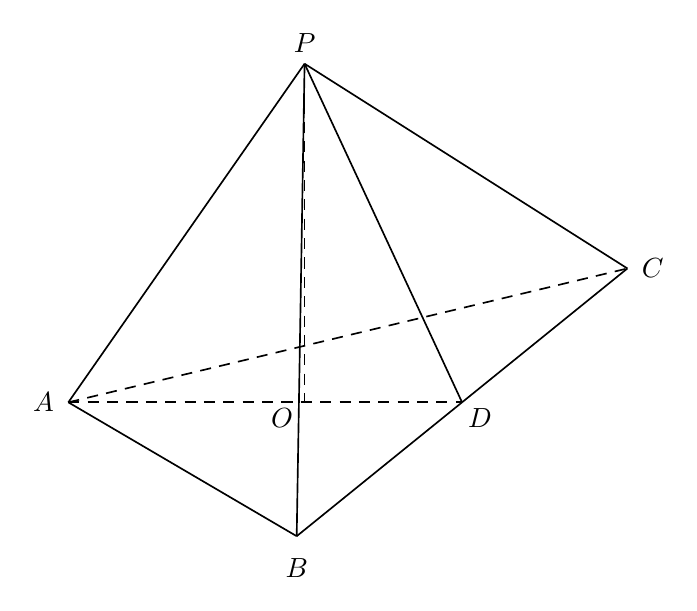
\begin{tikzpicture}[x=1cm,y=1cm,font=\normalsize,
  solid edge/.style={solid,line width=.6pt},
  hidden edge/.style={dashed,line width=.6pt,dash pattern=on 4pt off 3pt},
  geom label/.style={font=\normalsize,inner sep=2pt}]
\coordinate (P) at (-0.2,4.6);
\coordinate (O) at (-0.2,0.3);
\coordinate (A) at (-3.2,0.3);
\coordinate (D) at (1.8,0.3);
\coordinate (B) at (-0.3,-1.4);
\coordinate (C) at (3.9,2);
% base BC split at D (collinear B-D-C)
\draw[solid edge] (A) -- (B);
\draw[solid edge] (B) -- (D);
\draw[solid edge] (D) -- (C);
\draw[solid edge] (P) -- (A);
\draw[solid edge] (P) -- (B);
\draw[solid edge] (P) -- (D);
\draw[solid edge] (P) -- (C);
\draw[hidden edge] (A) -- (D);
\draw[hidden edge] (A) -- (C);
\draw[hidden edge] (P) -- (O);
\node[geom label,above,yshift=2pt] at (P) {$P$};
\node[geom label,left,xshift=-3pt] at (A) {$A$};
\node[geom label,below,yshift=-6pt] at (B) {$B$};
\node[geom label,right,xshift=3pt] at (C) {$C$};
\node[geom label,below right,inner sep=2pt] at (D) {$D$};
\node[geom label,below left,inner sep=2pt,xshift=-2.00bp,yshift=0.00bp] at (O) {$O$};
\end{tikzpicture}
